\section{Wearables}\label{sec:wearables} %Working title
%Hvad er en wearables / hvad er ikke en wearable
Wearable technology is a trending form of technology as of 2015. \todo{Find source; graph over how many devices every year?} As the name implies, wearables are devices that, unlike most electronics, are worn by the user. The most common types of wearables today are smartwatches, \ie watches that run an advanced operating system and can perform more actions that regular watches such as communicating with a smartphone or other smart devices, and smart wristbands which usually tracks activity, among other things, and sends this data to a connected smartphone via an application. Smartphones are usually not considered a wearable since they are usually \emph{carried} and not \emph{worn}. 

%Hvorfor wearables?
The increasing trend in wearables is likely due to increased computational power in small devices, decreased sizes of sensors, which allows more power and functionality to wearables devices, but also social acceptance of wearing such devices. \todo{Try to find sources confirming this} The increasing trend, as well as better wearables devices, opens up new possibilities since we can now carry more computational power with us on the go that we can utilize to perform actions that we could not before, or perform other actions faster or better. Examples of this could be that we can now track our level of activity together with our location to analyze ourselves or even automate actions based on our location, mood or even health. 

%HVad kan en wearable? Hvilke sensorer findes der? Hvad er state of the art? 
If we take a look at some of the current state of the art or the most popular wearable devices right now, we can create an image of what we can actually monitor, track, control or in other ways do with devices that we can wear. One of the latest and most advanced wearable is the HIRIS \cite{HIRIS}. The HIRIS is a wearable computer able to track 3D movements in real-time. By using several HIRIS, you can get a create a full-body tracking system. Aside from 3D tracking, HIRIS also tracks heart rate and temperature and can connect to other devices and control these. Another advanced wearable tracker is the Jawbone UP3 \cite{JAWBONE}. This wearable is also able to track your heart rate, activity, sleep and temperature, but unlike the Hiris cannot control any other devices. Since one of the most popular wearables is the smartwatch, it makes sense to mention these as well. One of most interesting smartwatches, due to developer options, is the Pebble Smartwatch \cite{PEBBLE}. This smartwatch works with iPhones and Android smartphones and comes with a variety of applications for tracking fitness and control music among other things. Aside from this, the watch also comes with an accelerometer and a magnetometer, meaning that is can track your motions and directions. 

By analyzing the list of wearables from Vandrico\cite{LISTOFWEARABLES} of September 2015, we can see which sensors are most common among wearables and where on the body they are worn. 
\todo{Make graphs of this}
\begin{figure}[!htb]
    \centering
    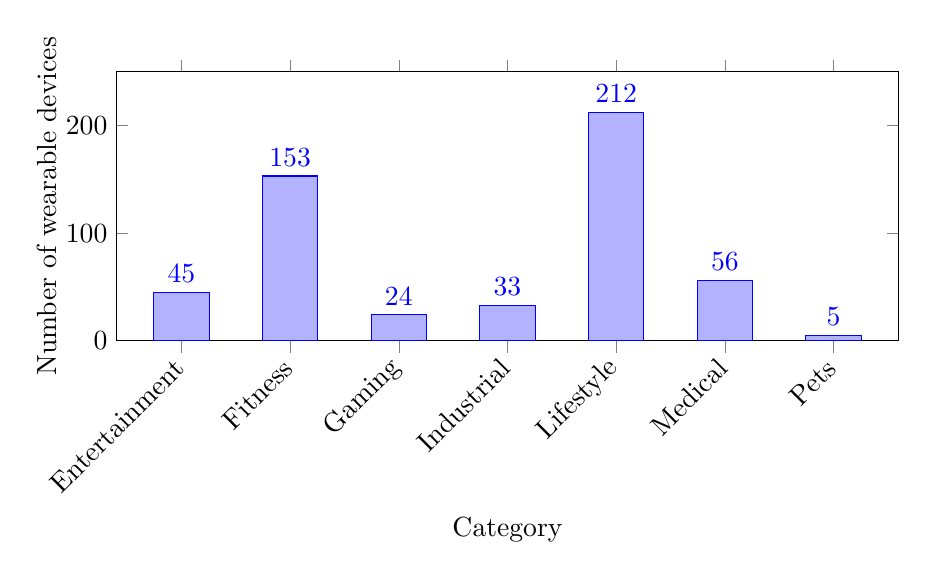
\begin{tikzpicture}
    \begin{axis}[
        height=5cm,
        width=0.95\textwidth,
        xlabel={Category},
        xticklabel style={rotate=45, anchor=east, yshift=-0.5ex},
        ylabel={Number of wearable devices},
        yticklabel style={align=right,inner sep=0pt,xshift=-0.3em},
        nodes near coords align={vertical},
        nodes near coords,
        xtick=data,
        symbolic x coords={Entertainment,Fitness,Gaming,Industrial,Lifestyle,Medical,Pets},
        ybar,
        ymax=250,
        ymin=0,
        bar width=20pt,
        ]
        \addplot coordinates {(Entertainment,45) (Fitness,153) (Gaming,24) (Industrial,33) (Lifestyle,212) (Medical,56) (Pets,5)};
    \end{axis}
\end{tikzpicture}
    \caption{Number of devices in each category}
    \label{fig:wearables-category}
\end{figure}

%Skab et overblik over de nyeste devices
%Grafer over hvilke sensorere der mest typiske?
%Grafer over kropsdele?
%Hvad er de nyeste teknologier indenfor wearables? 
